% !TeX spellcheck = en_GB 

\section{Results}
\begin{frame}
\frametitle{Results constant Dirichlet}
\begin{figure}[htp]
        \centering
        \makebox[\textwidth][c]{
        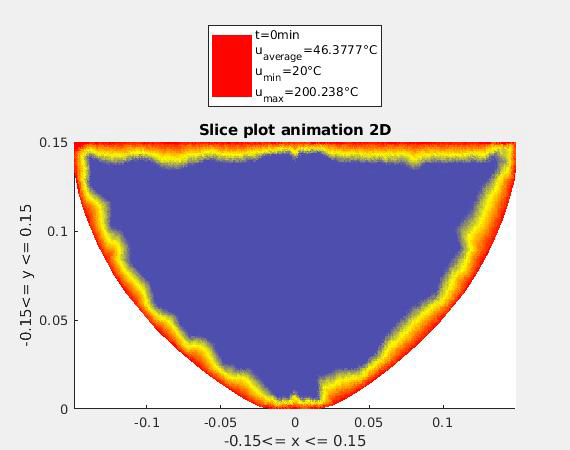
\includegraphics[width=0.37\textwidth]{figures/dirichlet_200_2D001.png}
        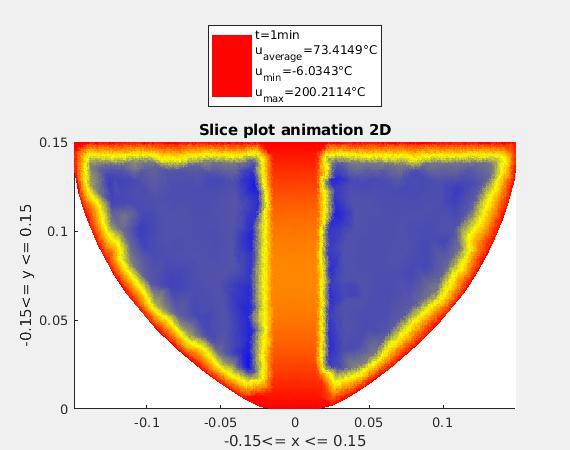
\includegraphics[width=0.37\textwidth]{figures/dirichlet_200_2D002.png}
        }
        \makebox[\textwidth][c]{
        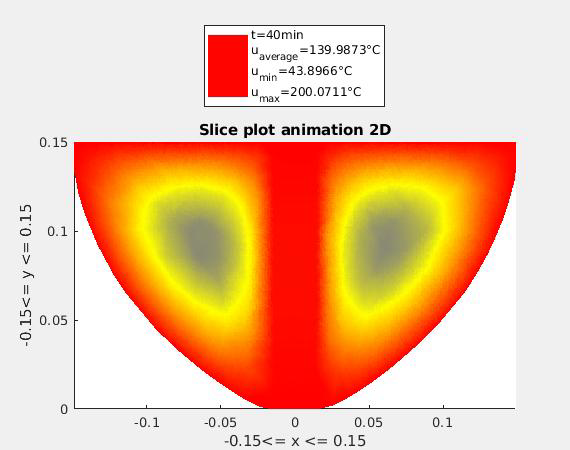
\includegraphics[width=0.37\textwidth]{figures/dirichlet_200_2D041.png}
        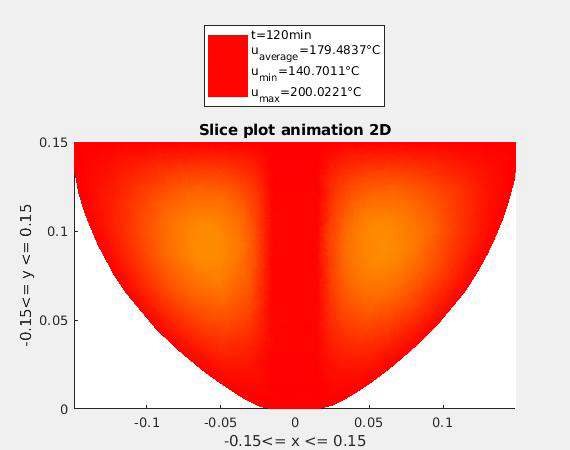
\includegraphics[width=0.37\textwidth]{figures/dirichlet_200_2D121.png}
        }
\end{figure}
\end{frame}

\begin{frame}
\frametitle{Results time dependent Dirichlet}
\begin{figure}[htp]
        \centering
        \makebox[\textwidth][c]{
        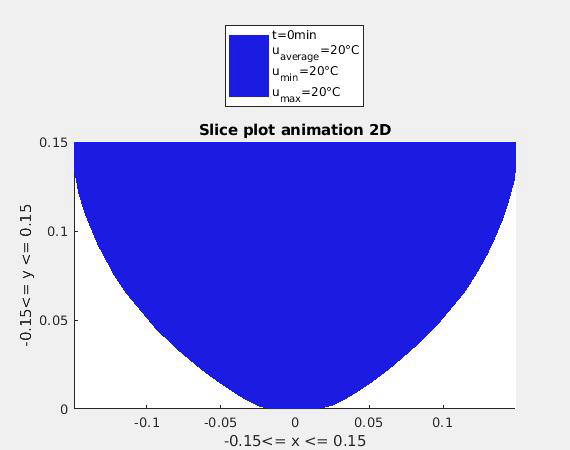
\includegraphics[width=0.37\textwidth]{figures/dirichlet_heat_200_2D001.png}
        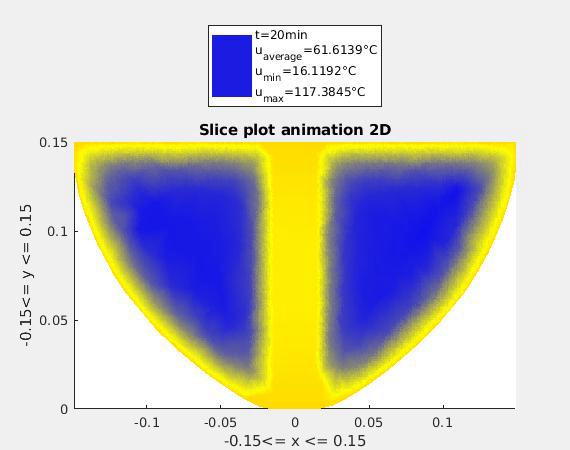
\includegraphics[width=0.37\textwidth]{figures/dirichlet_heat_200_2D021.png}
        }
        \makebox[\textwidth][c]{
        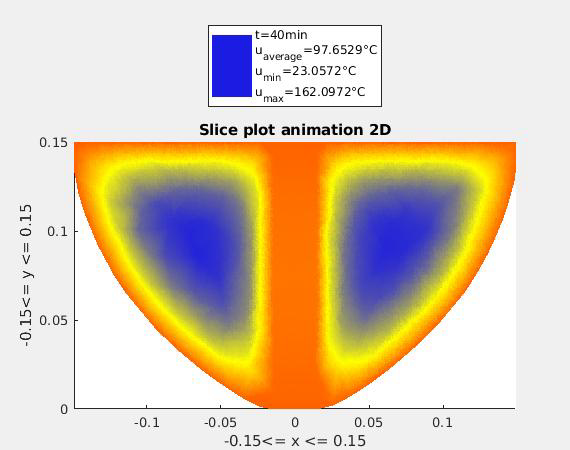
\includegraphics[width=0.37\textwidth]{figures/dirichlet_heat_200_2D041.png}
        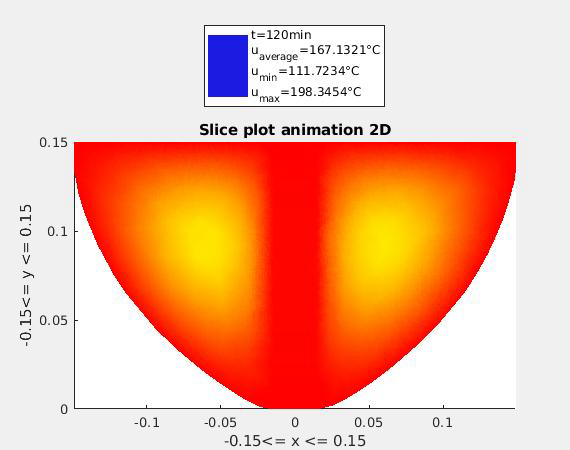
\includegraphics[width=0.37\textwidth]{figures/dirichlet_heat_200_2D121.png}
        }
\end{figure}
\end{frame}

\begin{frame}
\frametitle{Results Dirichlet without rod}
\begin{figure}[htp]
        \centering
        \makebox[\textwidth][c]{
        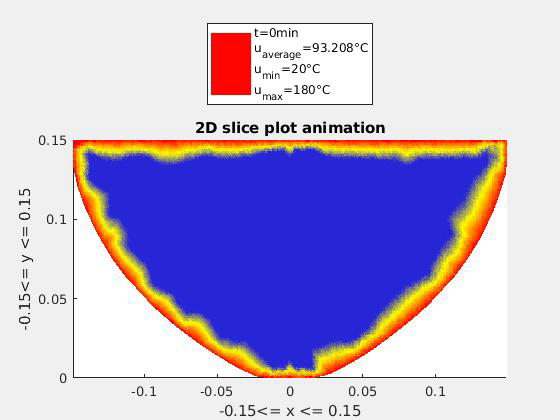
\includegraphics[width=0.37\textwidth]{figures/dirichlet_fullCake_2D001.png}
        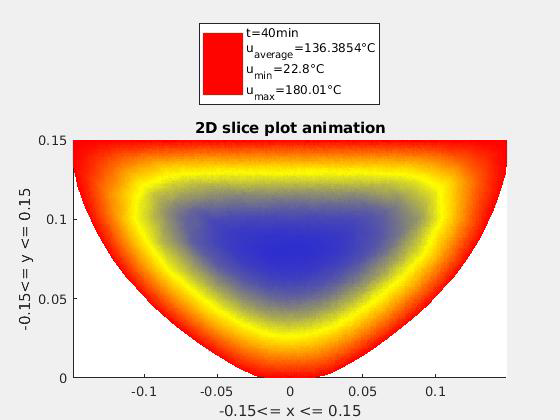
\includegraphics[width=0.37\textwidth]{figures/dirichlet_fullCake_2D041.png}
        }
        \makebox[\textwidth][c]{
        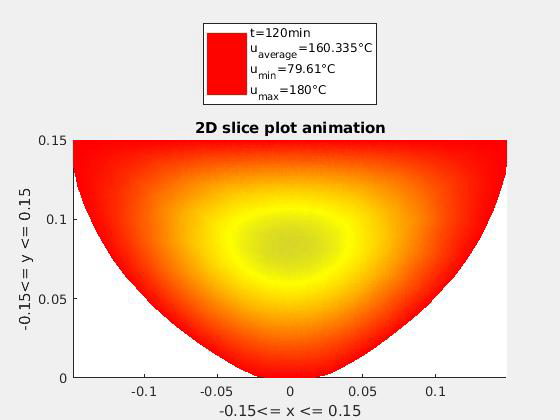
\includegraphics[width=0.37\textwidth]{figures/dirichlet_fullCake_2D121.png}
        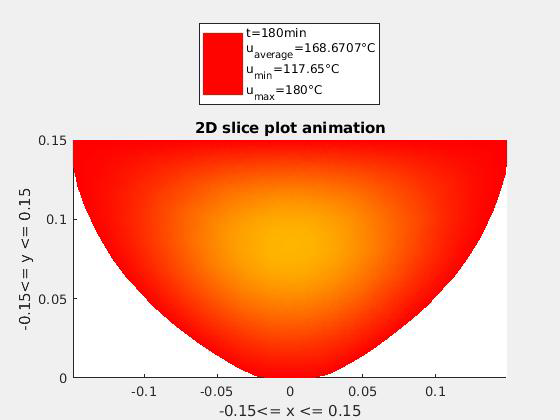
\includegraphics[width=0.37\textwidth]{figures/dirichlet_fullCake_2D181.png}
        }
\end{figure}
\end{frame}